\subsection{Dark matter and its connection to antinuclei}

\subsubsection{The evidence for dark matter}
\subsubsection{WIMP dark matter and the WIMP miracle}\label{sec:IntroWIMPs}
The WIMP miracle is well known to be the fact that when one considers a particle of the weak mass scale with a self annihilation cross section close to the weak interaction strength (on the pb level), the present day dark matter relic density can be obtained. Additionally, in many versions of supersymmetry, the lightest supersummetric particle is indeed a weakly interacting heavy particle, the ideal scenario for the WIMP\cite{}. In the following section the derivation of the WIMP abundance is shown, which is reproduced here from \cite{Baer-Choi-Kim}. The WIMP is denoted as $\chi$, and it is assumed be in thermal equilibrium with other matter while the Temperature is $T>$\dmm . During this time, the WIMP density $n_\chi$ evolves according to the Boltzmann equation, shown in equation \ref{eq:boltzman_deriv_eq}: 
\begin{equation}\label{eq:boltzman_deriv_eq}
    \frac{dn_\chi}{dt} = -3H n_\chi - <\sigma_{ann}v>(n_\chi^2 - n_{eq}^2)
\end{equation}
where H is the Hubble constant at that time, which in a radiation dominated universe is given by $H^2 = \rho_{rad}/3M^2_P$, where $M_P$ is the plank mass. While the system is in equilibrium, the number density tracks the equilibrium density $n_{eq}$. Subsequently, at some temperature $T_f$<m$_\chi$, the expansion rate will exceed the annihilation rate, and dark matter will freeze out, and their comoving number density (i.e. the number density accounting for the volumetric expansion of the universe) will remain constant from this point on. An approximate solution to the Boltzmann equation at this point gives equation \ref{eq:sol_Boltzmann}, where $\Omega_\chi h^2$ is the dimensionless dark matter density in the universe\footnote{$\Omega_\chi$ can be interpreted as the curvature of space which dark matter is responsible for.}, $s_0$ is the present day entropy density of the Universe, $g_*$ is the number of relativistic degrees of freedom of the particle $\chi$ at freeze out, and $x_f = T_f/m_\chi \approxeq 1/25$ is the freeze out temperature scaled to the dark matter mass. The value for $x_f=1/25$ is obtained from solving the Friedmann equation\footnote{This is the solution to Einstein's field equations for an open, closed or flat universe.} numerically for the freezeout Temperature (see \ref{Baer} for more details). This means that WIMPs would have still moved at relativistic speeds at freezeout, with velocities $<v>\approx c/3$. 

\begin{equation}
    \label{eq:sol_Boltzmann}
    \Omega_\chi h^2 \approx \frac{s_0}{\rho_c/h^2} \left( \frac{45}{\pi^2g_*}\right)^2 \frac{1}{x_f M_P} \frac{1}{<\sigma_{ann}v>}
\end{equation}

Plugging in the known values for the parameters\cite{ref 533 DM review} and setting $\Omega_\chi h^2$ = 0.12 from the latest Planck Collaboration results \cite{Planck2018}, one obtains equation \ref{eq:DM_relic_density}. 

\begin{equation}
    \label{eq:DM_relic_density}
    \frac{\Omega h^2}{0.12} = \frac{1}{<\frac{\sigma_{ann}}{10^{-36} cm^2} \frac{v/c}{0.1}}
\end{equation}

Thus, setting the thermally averaged annihilation cross section to a value of 1pb * $c$, and using average velocities of the order one would expect from a WIMP at freezeout, the current dark matter abundance is recovered. A schematic representation of this process is shown in figure \ref{fig:DM_thremal_eq_freeze_out}, where the decoupling temperature $T_{dec}$ and the freezeout temperature $T_{f}$ are shown separately. The decoupling temperature is the temperature at which the dark matter and luminous matter stop being in thermal equilibrium, while the freeze out temperature the point where the expansion rate becomes the dominant term for the density change for dark matter, over the annihilation term. 

\begin{figure}[htbp]
    \centering
    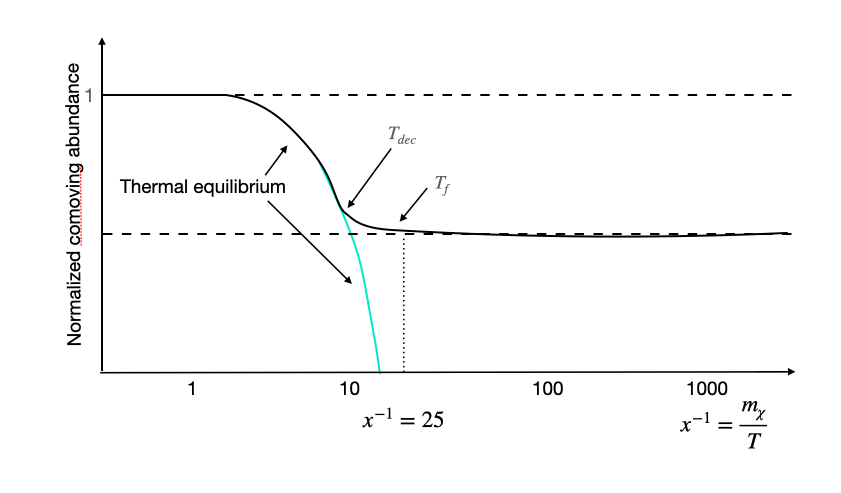
\includegraphics[width=\textwidth]{figures/schematic_thermal_eq_evolution_DM.png}
    \caption{Transition of dark matter from thermal equilibrium to freeze out. Both the decoupling temperature (where dark matter stops being in thermal equilibrium with luminous matter) and the freeze out temperature (when the rate of expansion has dropped the annihilation rate to negligible amounts, so that the comoving density can be considered constant) are indicated on the schematic. Figure is based on the figure in \cite{Baer}}
    \label{fig:DM_thremal_eq_freeze_out}
\end{figure}



\subsubsection{Other dark matter models}\label{IntroOtherDM}
WIMP dark matter is not the only dark matter model on the market, indeed, dark matter models span over $\approx$ 30 orders of magnitude in mass. A collection of models and their mass ranges is shown in figure \ref{fig:DarkMatterModelsSummary}. Notable other dark matter candidates are neutrinos, sterile neutrinos, axions and primordial black holes (not shown in figure \ref{fig:DarkMatterModelsSummary}). In this section we shall briefly discuss their main concepts, advantages and disadvantages. Promising candidates usually share the quality that they solve not just the nature of dark matter, but also another problem in physics. As discussed earlier, the WIMP neutralino was considered the supersymmetric extension to the standard model at its inception.\\

\begin{figure}[bthp]
    \centering
    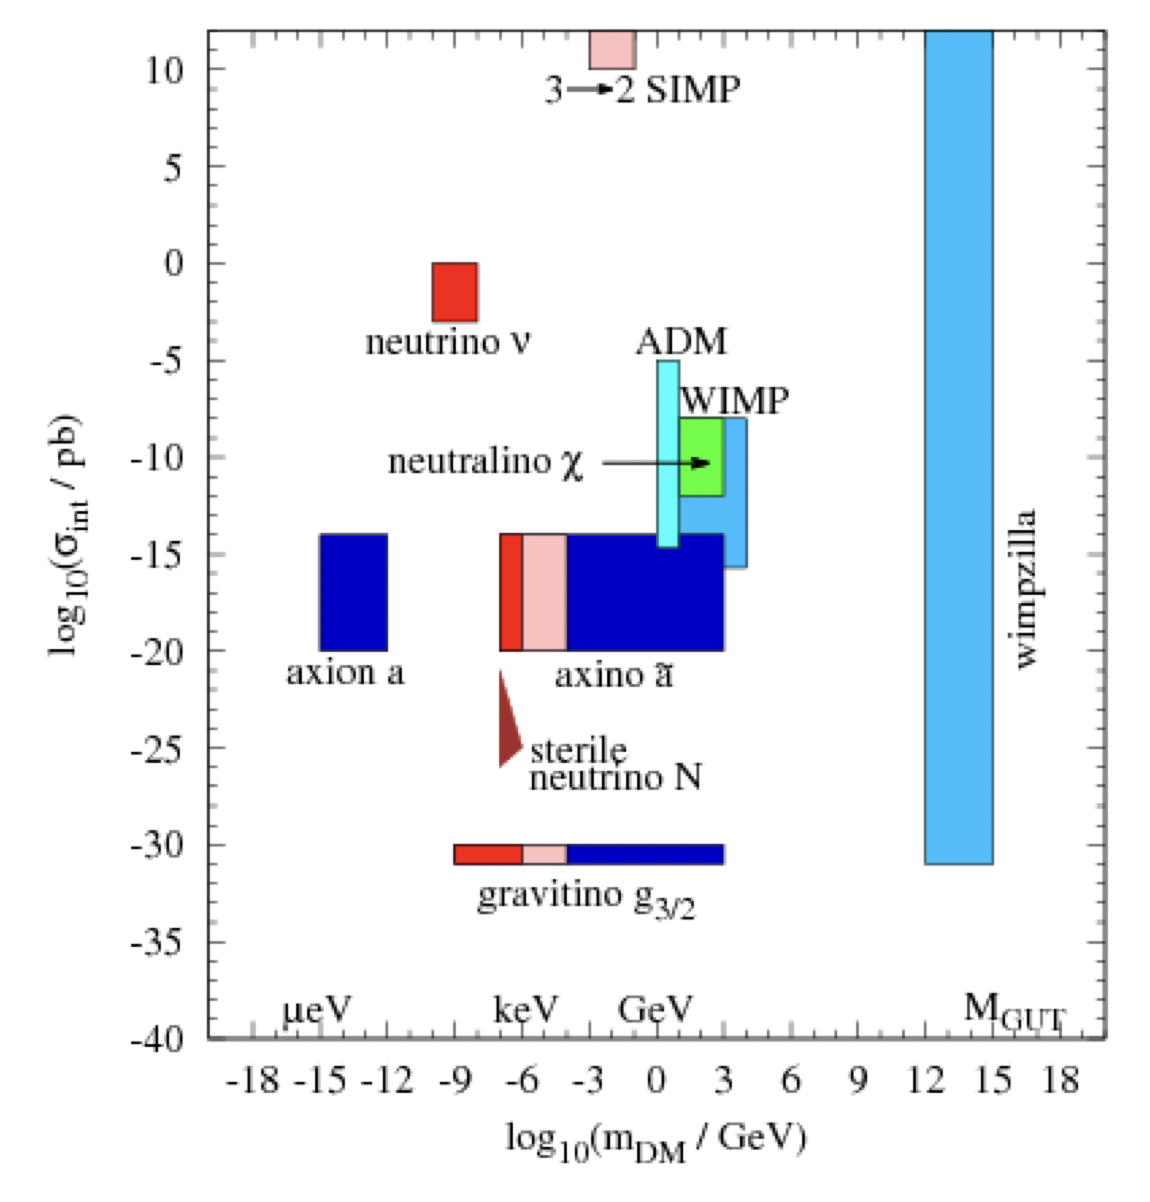
\includegraphics[width=\textwidth]{figures/DM_summary_models.png}
    \caption{Collection of candidate dark matter models over a wide mass range. The most prominent candidates are WIMP dark matter, axion dark matter and sterile neutrinos. Primordial black hole dark matter is not shown on this plot. Figure taken from \cite{BAER20151}.}
    \label{fig:DarkMatterModelsSummary}
\end{figure}

Let us first consider axion dark matter. Axions arise naturally in the Peccei-Quinn (PQ) solution to the strong CP problem\cite{PQ_axion, Weinberg} (see section \ref{sec:IntroSymmetries} for more details), by arguing that the CP violating term $\bar{\theta}$ of the QCD Lagrangian is relaxed to 0 due to an additional PQ symmetry. This symmetry is accompanied by a scalar field which spontaneously breaks the symmetry at low energy, giving rise to the axion. While the initial model, which predicted axion masses of order O(100keV) has long since been experimentally ruled out, it has been replaced by models using the same mechanism to dynamically solve the strong CP problem. Axions of such fields are expected to have masses in the $\mu$eV range. As a side effect, the scalar field would populate the universe with axions, which since they are produced non-thermally at rest\cite{cookbook} would be considered cold dark matter even though they have such low masses. As such, and dark matter theory which is not at least partially made up of axions has to provide an alternate solution to the strong CP problem. It's mass can be constrained from the top by \\

Out of all the standard model particles, the neutrino is the only particle which does not interact through either the strong or electromagnetic forces. This makes it a plausible 

talk about:
- axion DM
- sterile neutrinos
- range of masses
- pbhs

\subsubsection{Dark matter annihilations into antinuclei}
\subsubsection{Majorana vs. Dirac dark matter}\label{sec:IntroMajoranaDiracDM}
Since the properties of dark matter are not know beyond its gravitational pull, it is also not known if dark matter is its own anti-particle. 
\subsubsection{The distribution of dark matter within our galaxy}
\subsubsection{The search for dark matter: the link between WIMP dark matter and antinuclei}